\section{Planteamiento del Problema y Solución Propuesta} \label{sect:planteamiento_solucion}

Actualmente \textit{Tuguia.de} cuenta con funcionalidades tales como búsqueda de locales dadas sus ubicación y/o una serie de taxonomías asociadas a éstos, además siempre que se muestra información de un local se debe mostrar su ubicación en el mapa, dirección, fotografías asociadas e información de contacto. Un aspecto importante para la visión de negocio de \textit{Tuguia.de} es la capacidad de que los usuarios puedan realizar comentarios y establecer una puntuación de uno a cinco  sobre los locales, esto con el objetivo de brindar no solo la información básica de un establecimiento, sino también priorizar los locales de acuerdo a la opinión de los usuarios. Adicionalmente, \textit{Tuguia.de} prevé ofrecer la posibilidad a los dueños de cada local de gestionar la información de su comercio y campañas de publicidad en el sitio.

El Proyecto de pasantía consiste en llevar las funcionalidades presentes a una aplicación móvil para el sistema operativo Android, agregando nuevas funcionalidades aprovechando los elementos propios de los teléfonos inteligentes como geolocalización y así realizar búsquedas usando la posición actual del equipo y de esta forma brindar información más precisa a los usuarios de \textit{Tuguia.de}.

Para exportar la funcionalidad de \textit{Tuguia.de} se desarrolló un API (Aplication Programming Interface), que permite gestionar el contenido de la página a través de él. La aplicación móvil debe usar este API como materia prima para realizar sus operaciones y de esta manera mantener comunicación constante con la aplicación de \textit{Tuguia.de} para mantener el contenido siempre actualizado.

La figura \ref{fig:AndroidVersion} muestra la distribución de equipos por sistema operativo.  

\begin{figure}[h]
	\begin{center}
		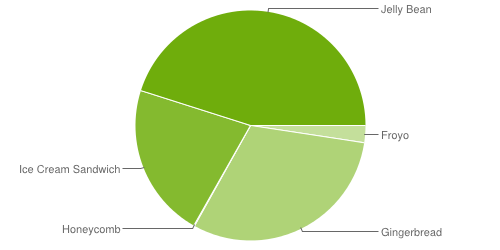
\includegraphics[scale=0.5]{imagenes/chart.png}
	\end{center}
	\caption{
		\label{fig:AndroidVersion}
		Distribución de dispositivos Android por sistemas operativos.
	}
\end{figure}

Se espera que la aplicación móvil, pueda operar efectivamente en las diferentes versiones activas de Android, al menos en las que concentran la mayor cantidad de usuarios. Además debe tener un uso mínimo de la red de datos y poseer una interfaz sencilla y fácil de usar.

